\documentclass{ctexart}
\usepackage{graphicx}
\usepackage{float}
\usepackage{caption}
\usepackage{tikz}
\begin{document}
	\title{“Moon”企划}
	\author{张乐平}
	\date{2022年10月25日}
	\maketitle

	\abstract{这是一个星际探索游戏的制作企划,主题在于想要体现古希腊式的“必然实现的悲剧”。人类再一次失去原始纽带,向着没有尽头的太空深处无止境的前进,体会未知与陌生的恐惧。}
	\tableofcontents
	\newpage
	\section{玩法综述以及制作流程设计}
		\subsection{基于直线的树状流程:DeathTrip to Canda}
		玩家需要以有限的资源,操纵飞船进行横向前进,在有限的时间内,抵达预先设定的目的地。飞船运行时会逐渐消耗耐久度,需要资源进行维修,主角的在飞船上的生存也需要消耗资源。

		物资在一开始有部分存量,之后需要在未知的星球上探索来获取。如果选择一直向右探索,虽然会有资源点,但是获得的资源非常少,仅仅能够在运气好的情况下勉强来到目的地,但是不需要花费很多时间。因此,为了补充资源,玩家可以选择不继续前进,向上下探索资源点来获取物资继续前进,并且可以结识一些NPC推动剧情,获取装备或者是强化道具,但是需要花费时间。
		
		不会以直接战斗的形式让玩家打怪,而是在根据玩家的装备属性在探索时触发事件。
		\subsection{游戏点}
			\subsubsection{剧情推动的多周目探索}
		主角一开始是以失忆的状态进入太空,只知道自己的目的就是前往某个在地图上出现的目标点,在与人沟通时会逐渐理解游戏的剧情。	
		
		游戏有时间限制,玩家不可能每个NPC都做完所有的剧情任务,因此需要多周目游玩才能完整的知道游戏剧情。知道自己为什么会来到这无人深空。
		
		NPC们似乎都是为了逃离在战乱、瘟疫中的母星,而与主角相遇。
				
		如果玩家完全没有触发NPC的剧情事件,那么就是主角实现了自己一开始的愿望,然后在郁郁葱葱的草地上睡去,在家乡战火的噩梦中惊醒。“梦醒”
		
		而如果玩家只是了解了部分剧情,那么游戏的理解就会是建立了新的家园,从失去家到有了新的家。“逃离”
		
		主角在到达目的地后,当玩家游玩过所有剧情就会知道,主角的使命是为了拯救,拯救母星而不是逃离母星,在目的地放弃安全的环境与充足的资源。可是,返航的路是十分困难的,在返航途中,遇到过的NPC会拆解自己的飞船,拼装到主角的飞船上,舍弃自己所有的装备、资源贡献给主角,让他继续前进,成功拯救家园。“返航”
			\subsubsection{目标与羁绊的取舍}
		游戏开始的目标即为前往目标点,玩家可以选择以最近的路线直线前往目的地,这样会因为资源匮乏而难度很大,但是能够有效的节约回合数,有更加充足的时间。
			
		在游玩的过程中也可以选择绕远路探索,会花费很多时间和燃料前往物资更多的星球。并且有概率遇到NPC,NPC会与玩家建立羁绊关系,并且给玩家一些道具和装备。需要玩家自省什么才是真正重要的东西。可以选择跟NPC在一起,而不再前往一开始被定义的终点。
			\subsubsection{回合制随机事件}	
		游戏并不是线性的时间流逝,而是以回合来推动时间流动。根据玩家所在区域、资源数量、NPC剧情进度在每个回合会触发随机事件。并且使用类似dota的暴击设定,伪随机防止好事件和恶性事件连续出现。
		
		NPC剧情事件也有固定触发和随机触发两种,有些关键NPC是必定触发的,而其他的会在指定区域概率出现,当然,见不到也应该有补救的措施。增加了重复游戏的可能性。	
		
		采用回合制降低了玩家的操作要求,转而需要玩家进行大脑的思考,算某种程度上降低游玩门槛。并且降低游戏的制作复杂度。
			\subsubsection{路线的搭配与选择}
			虽然地图是固定的,但是由于不同NPC会给不同的帮助或者说是加护,玩家需要选择不同的搭配方式进行组合,找出最优解。
			\section{系统界面及其实现方式}
		考虑到制作成本和时间的难度,选择使用2D的游戏画面。为了体现宇宙的神秘感,应该使用高px像素画或者是直接用2d绘图。以下为UI界面设计和摆放位置的参考。要有科技感的界面。
		参考图1至3的界面UI。
		\begin{figure}[H]
			\centering
			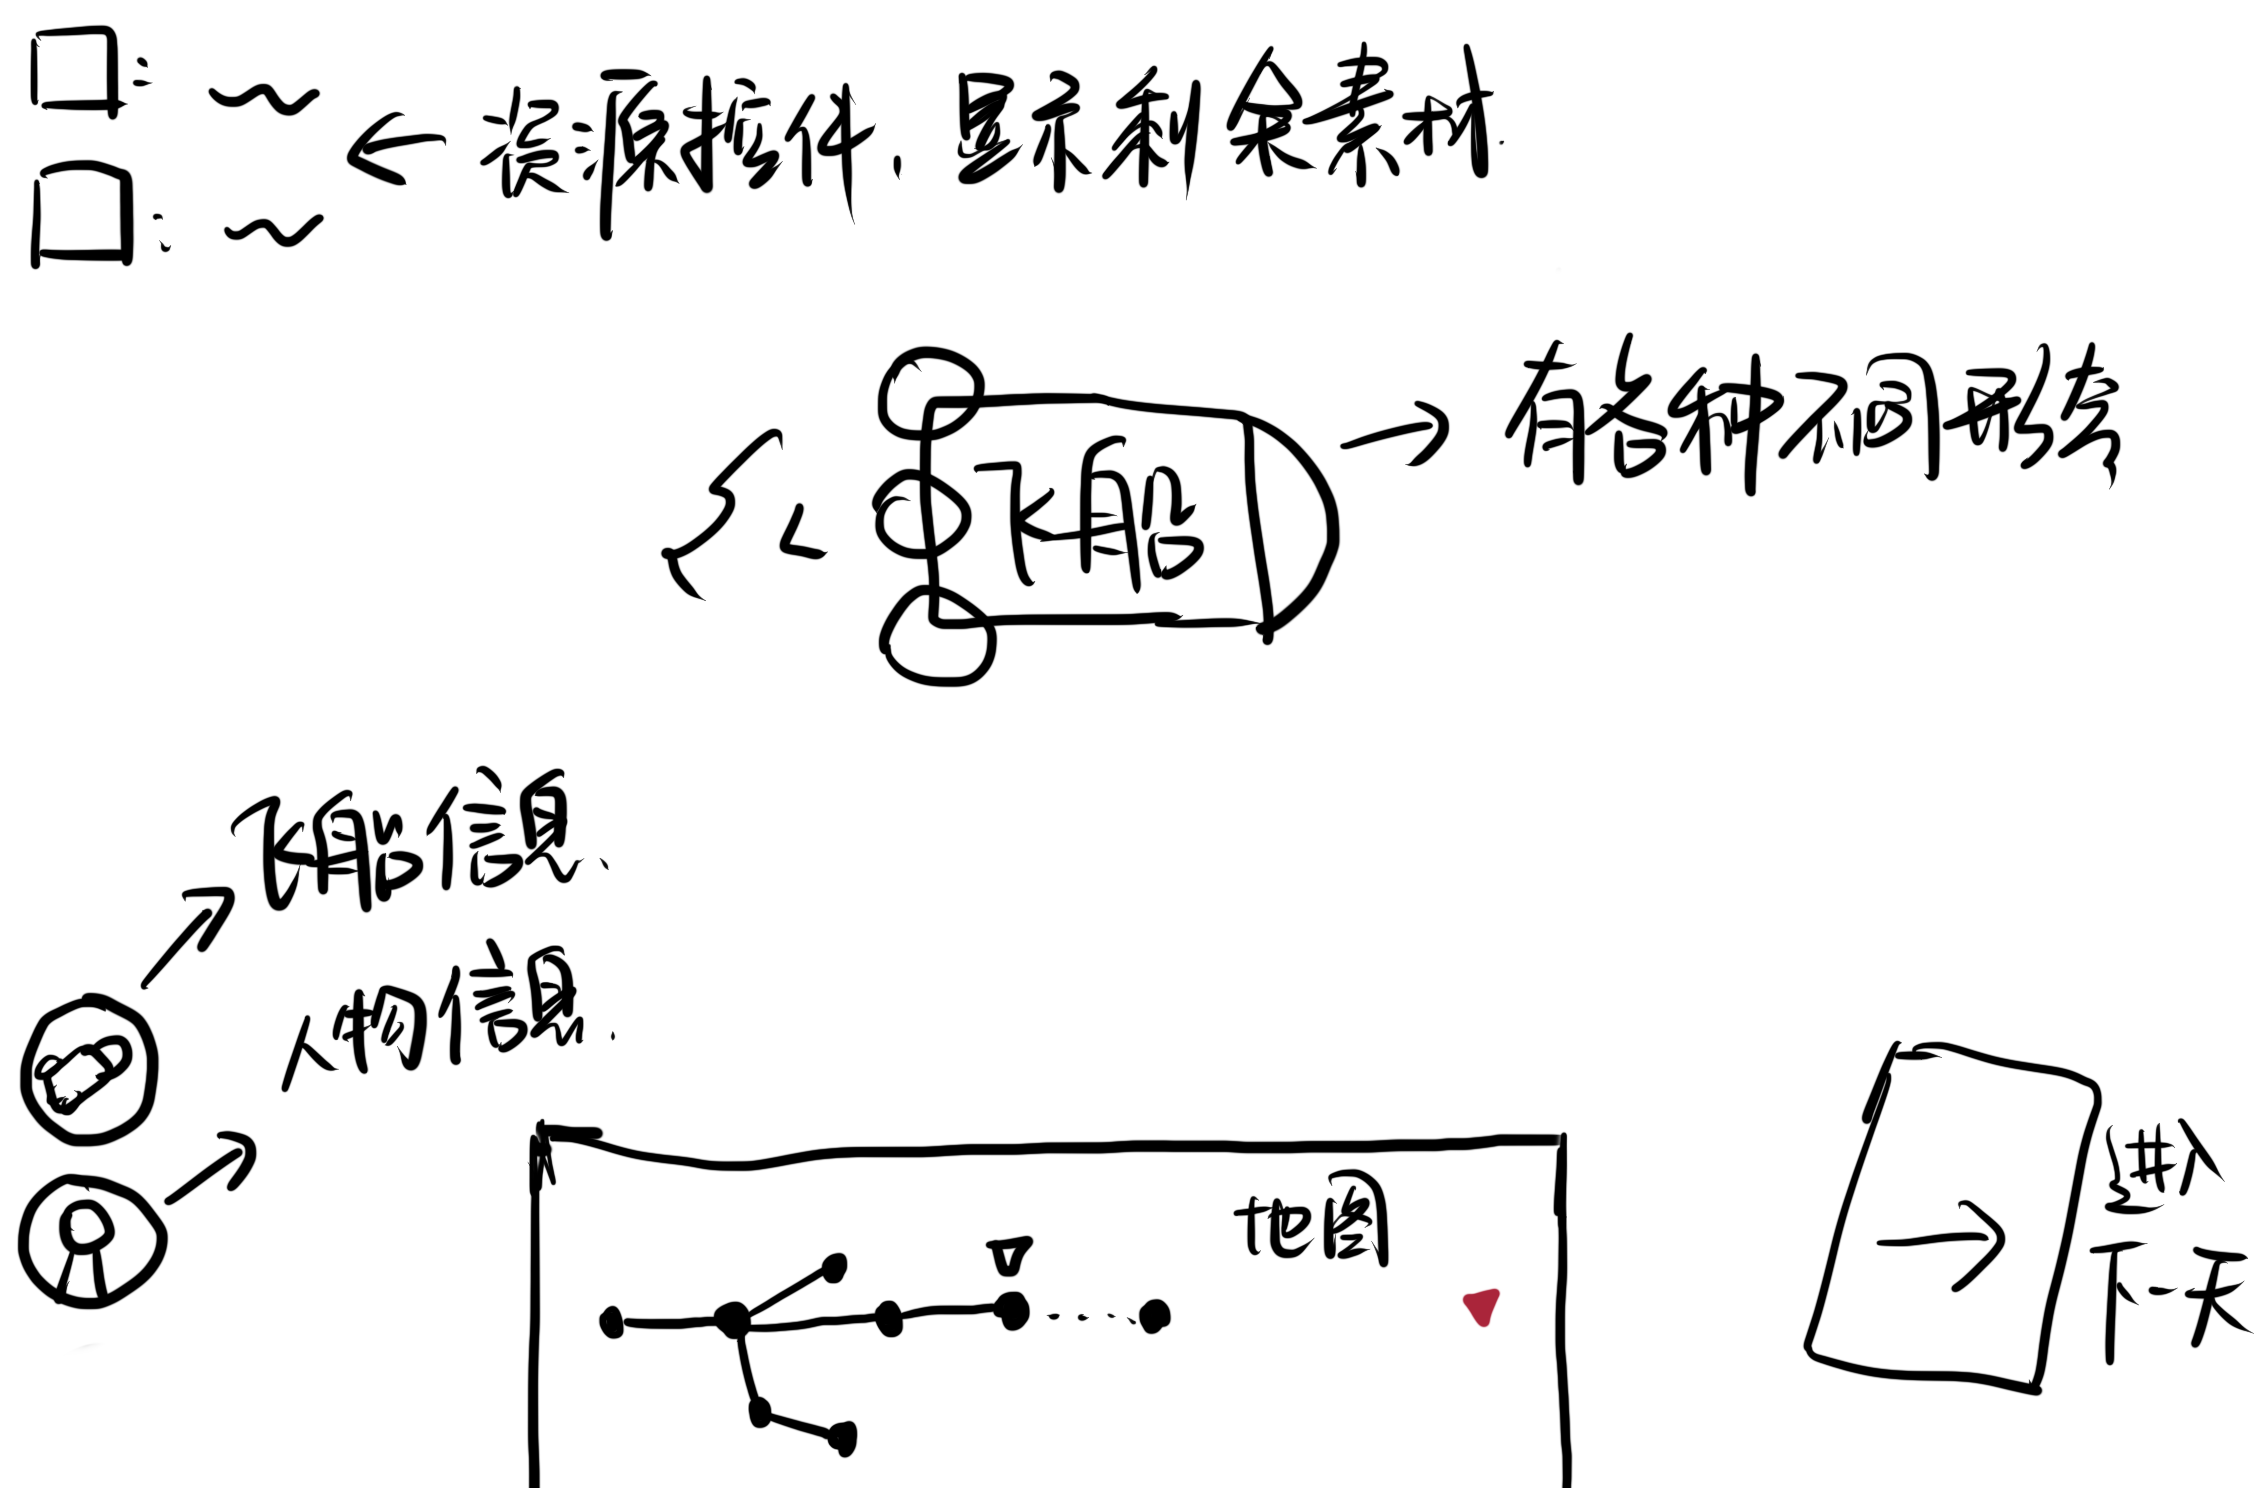
\includegraphics[scale=0.2]{material/整体界面UI.png}
			\caption{整体界面UI}
			\label{整体界面UI}
		\end{figure}
		
		\begin{figure}[H]
			\centering
			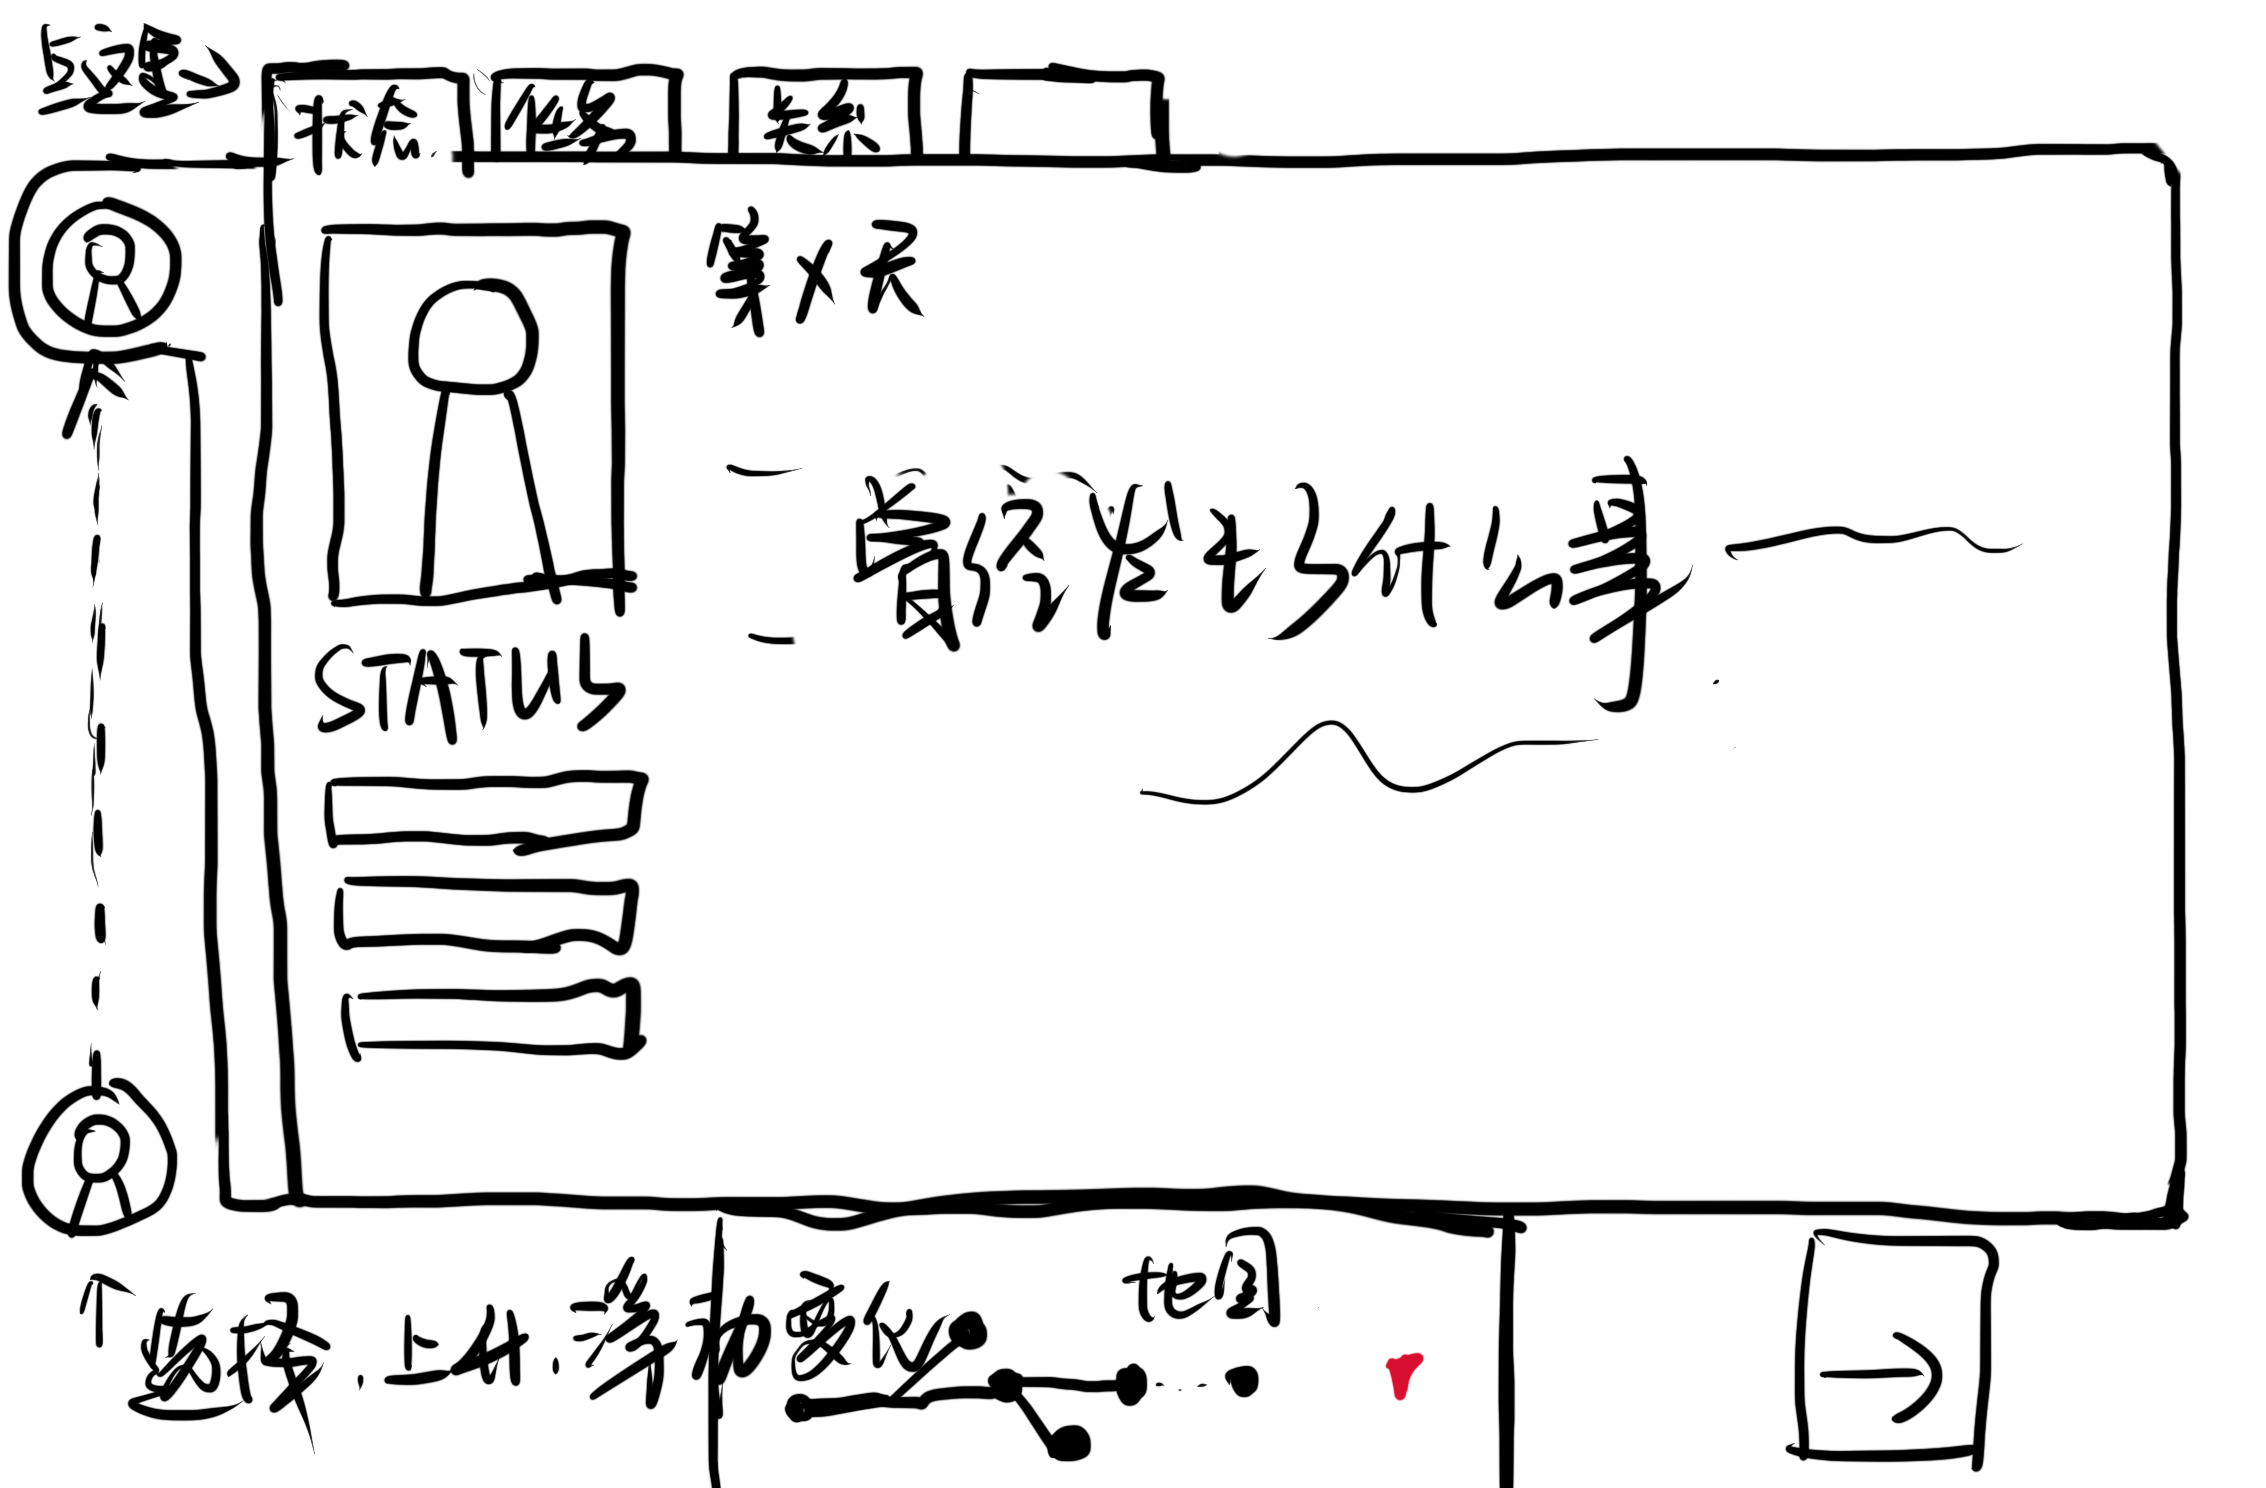
\includegraphics[scale=0.2]{material/人物属性UI.png}
			\caption{人物属性UI}
			\label{人物属性UI}
		\end{figure}
		
		\begin{figure}[H]
			\centering
			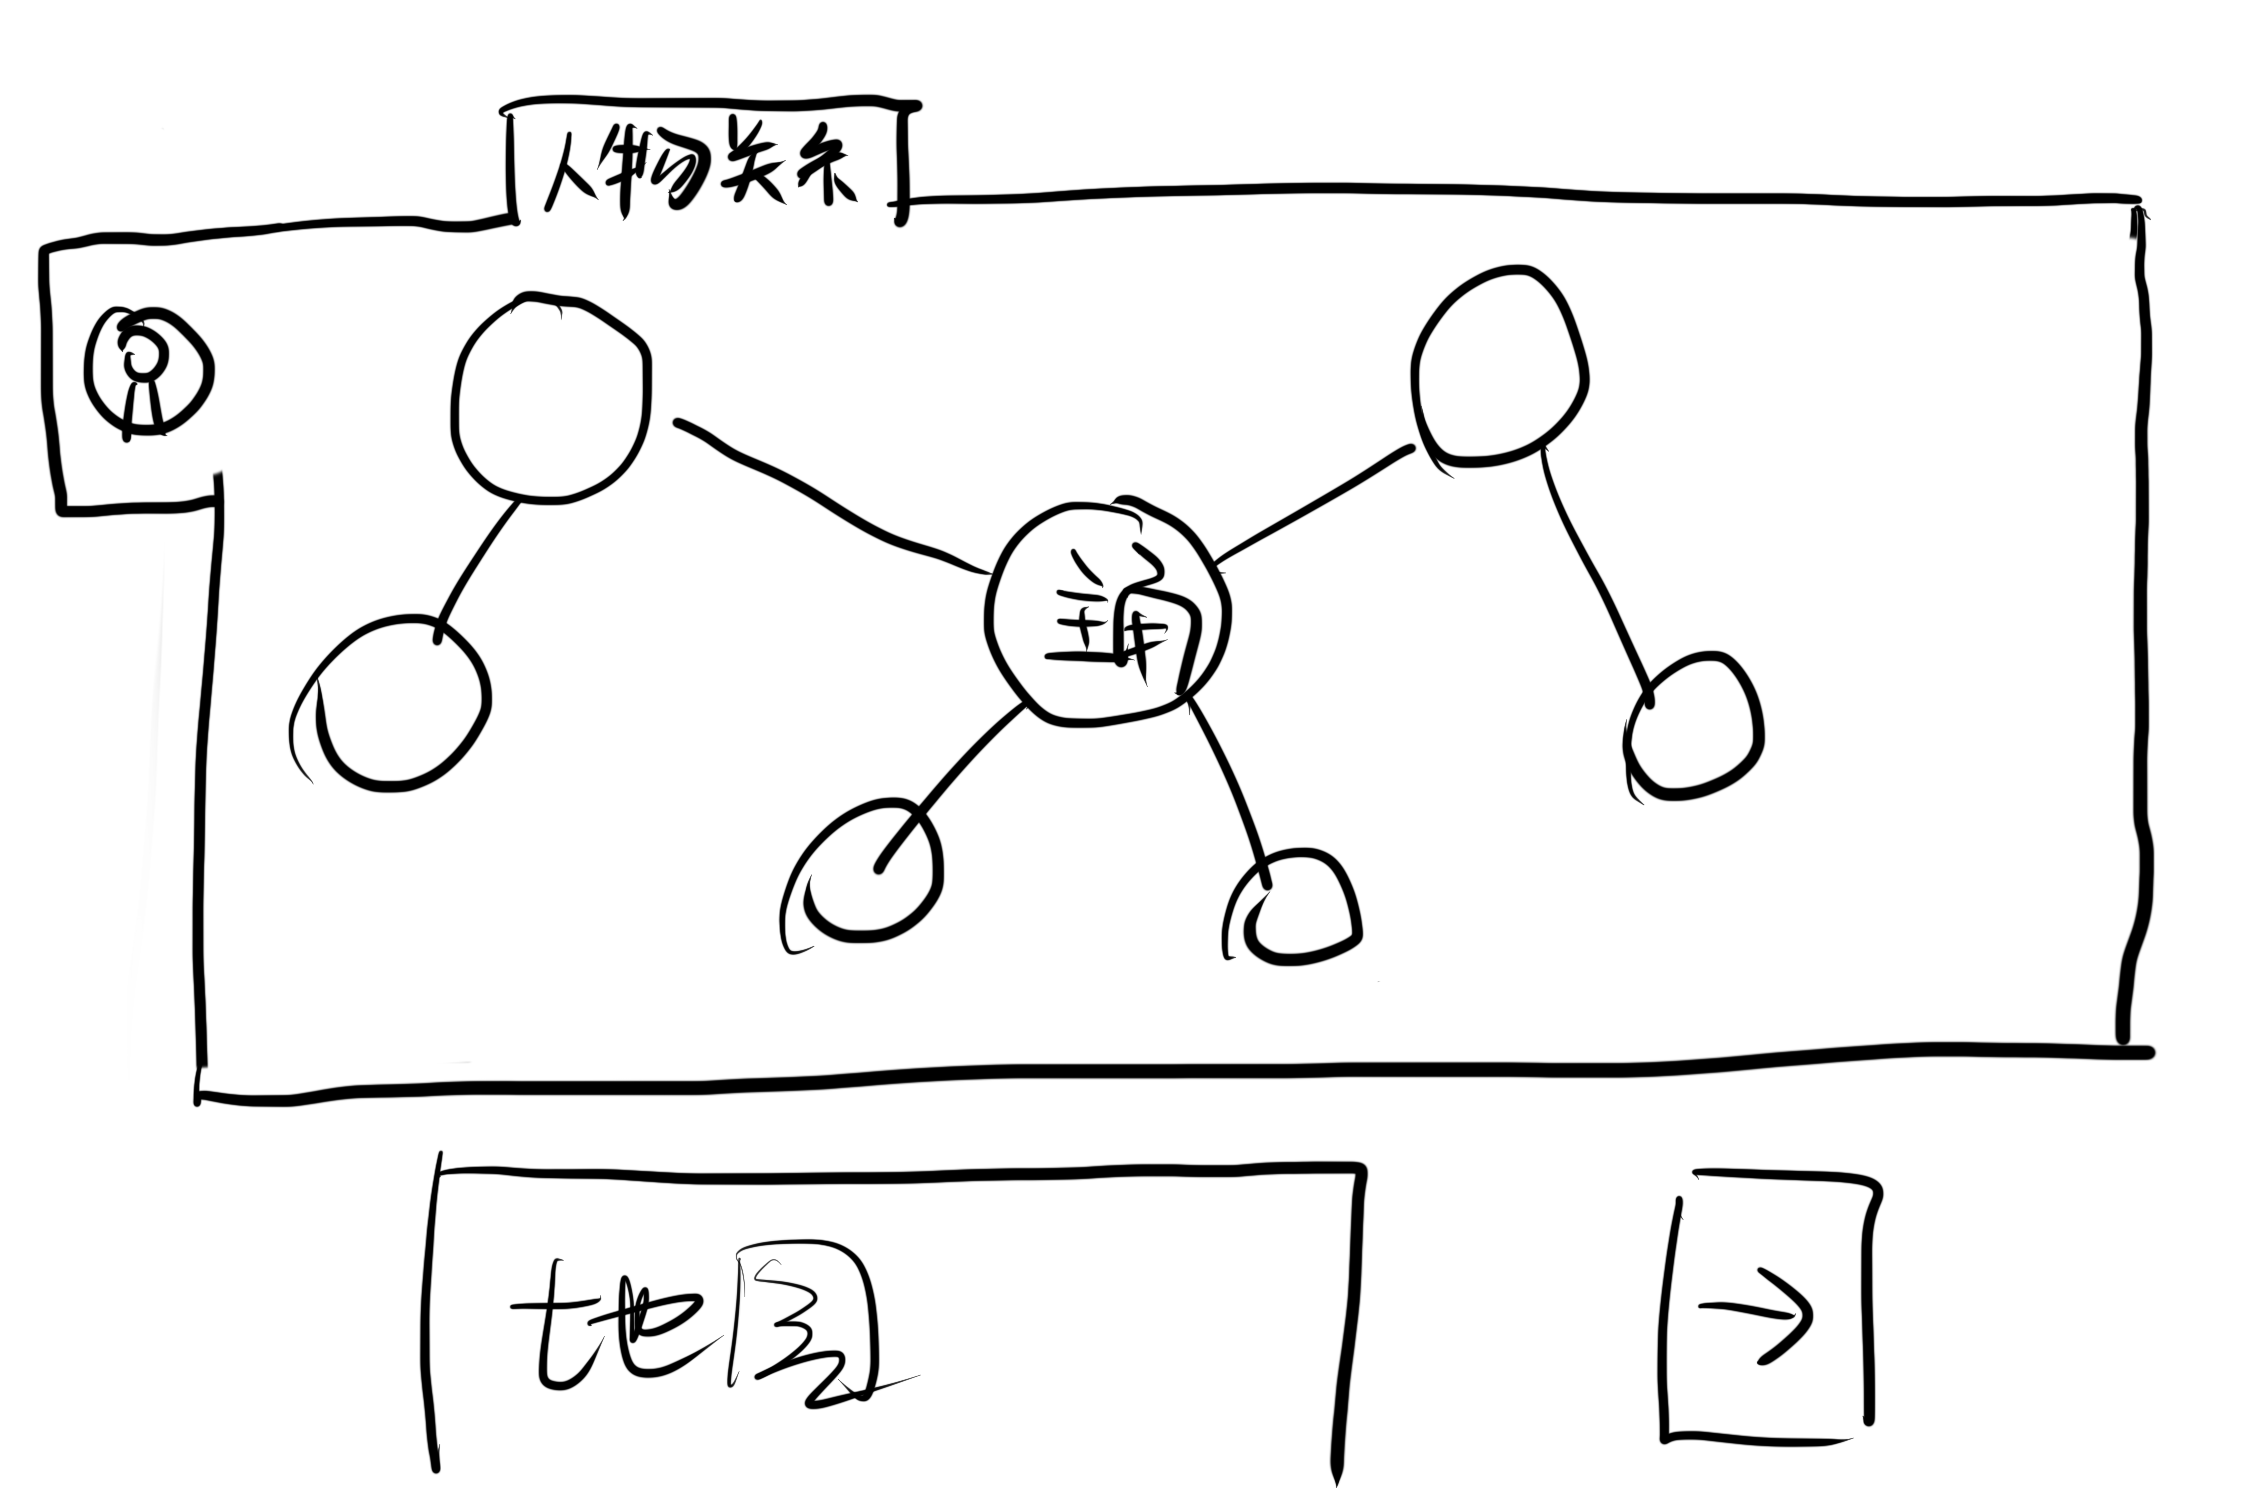
\includegraphics[scale=0.2]{material/人物关系UI.png}
			\caption{人物关系UI}
			\label{人物关系UI}
		\end{figure}
		
		% TODO 在这里要加上开始界面的UI和进入游戏的选择界面
	\section{美术、音乐风格选择}
		\subsection{音乐构成}
			\begin{enumerate}
				\item 本体BGM:在游戏过程中一直循环播放,一旦有事件发生则切换为别的音乐。最长
				\item 探索BGM:探索资源、采掘资源时播放
				\item 战斗BGM:在发生战斗事件或者什么不好的事件的时候播放
				\item 角色BGM:在与NPC对话时播放,或者角色在自说自话时播放
				\item 以及各种音效,比如敲矿物之类的声音
			\end{enumerate}
		\subsection{美术风格}
			\subsubsection{剧情对话与事件界面}
			有较高精度像素人物,如下是界面摆放位置参考。需要绘制主角以及剧情NPC的人物像。
			\begin{enumerate}
				\item 每个NPC需要一张立绘,并且有三种不同的表情形态,即可只修改面部表情即可
				
				\begin{figure}[H]
				\centering
				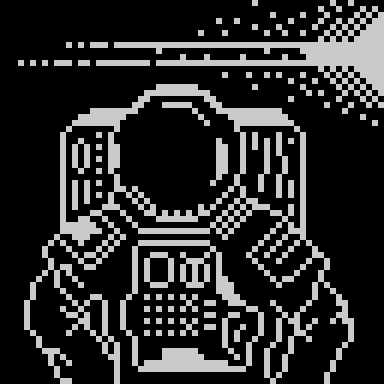
\includegraphics[scale=0.4]{material/宇航员.png}
				\caption{人物头像(测试版)}
				\label{人物头像}
				\end{figure}
				\item 心情的气泡图像,分别为“!”“?”“、、、”和“**”(开心)这几种,之后可能会再加,用来调整对话节奏和剧情
				\item 人物对话框已经绘制完毕,直接修改边框为每个人独特的颜色即可,注意的是那个声音波形是要做成动画的 
				\begin{figure}[H]
				\centering
				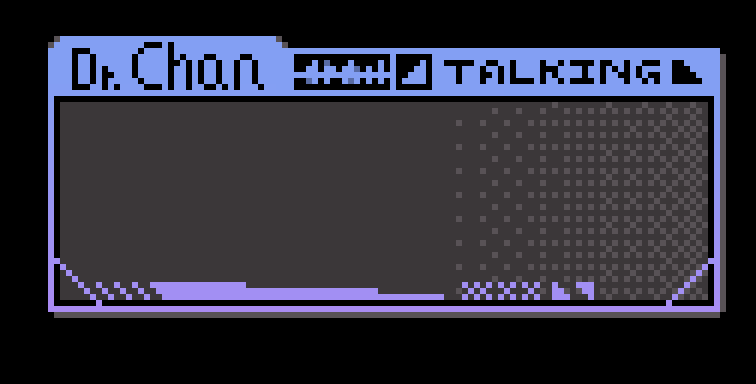
\includegraphics[scale=0.4]{material/hud3.png}
				\caption{人物对话框}
				\label{人物对话框}
				\end{figure}
				\item 事件对话框应该也算画完了,但是像素尺寸可能要修改的大一点,现在那个只能说是事件的提醒界面
				\begin{figure}[H]
				\centering
				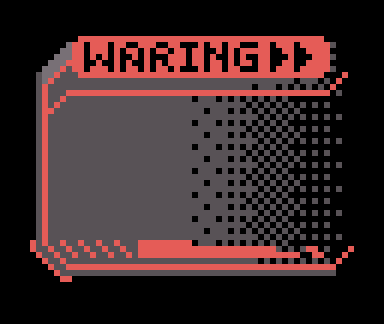
\includegraphics[scale=0.4]{material/hud2.png}
				\caption{事件警告提示}
				\label{事件警告提示}
				\end{figure}

				\item 每种大类的事件是有不同的图的,这个图也要画,就比如天灾、人祸分类
				\item 人物在对话的时候有运动特效和相应的情绪音效,可以参考碧蓝档案
			\end{enumerate}
			\begin{figure}[H]
			\centering
			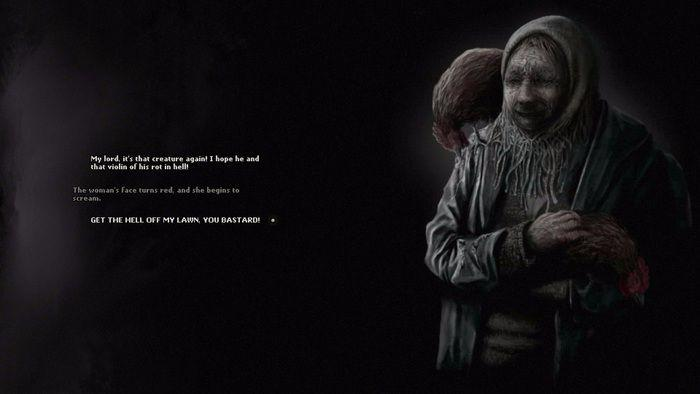
\includegraphics[scale=0.4]{material/美术参考人物1.jpeg}
			\caption{darkwood参考}
			\label{darkwood参考}
			\end{figure}
			\subsubsection{界面UI参考}
			\begin{figure}[H]
				\centering
				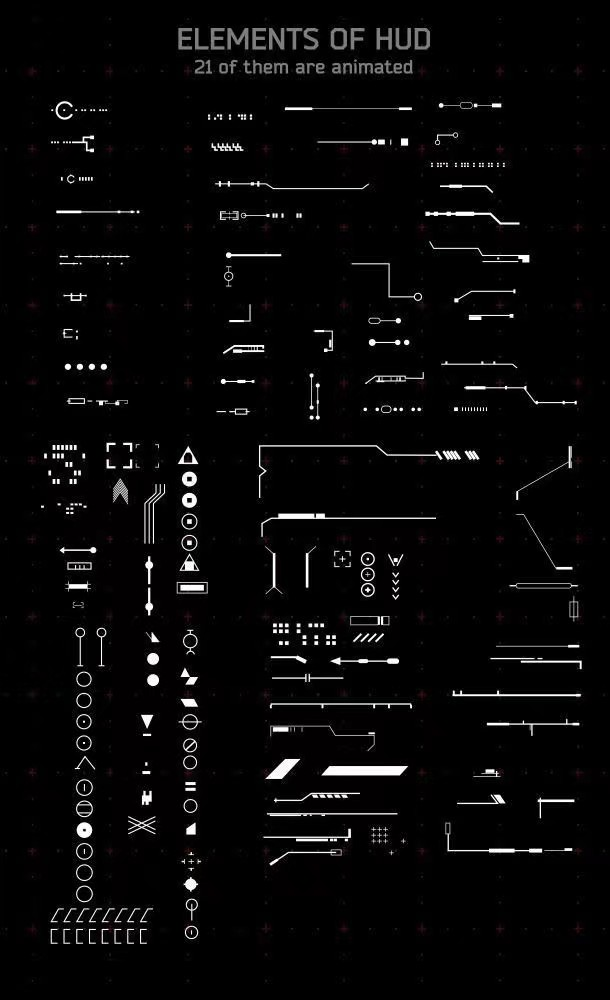
\includegraphics[scale=0.6]{material/UI设计参考1.jpeg}
				\caption{UI地图绘制参考}
			\end{figure}
			\begin{figure}[H]
				\centering
				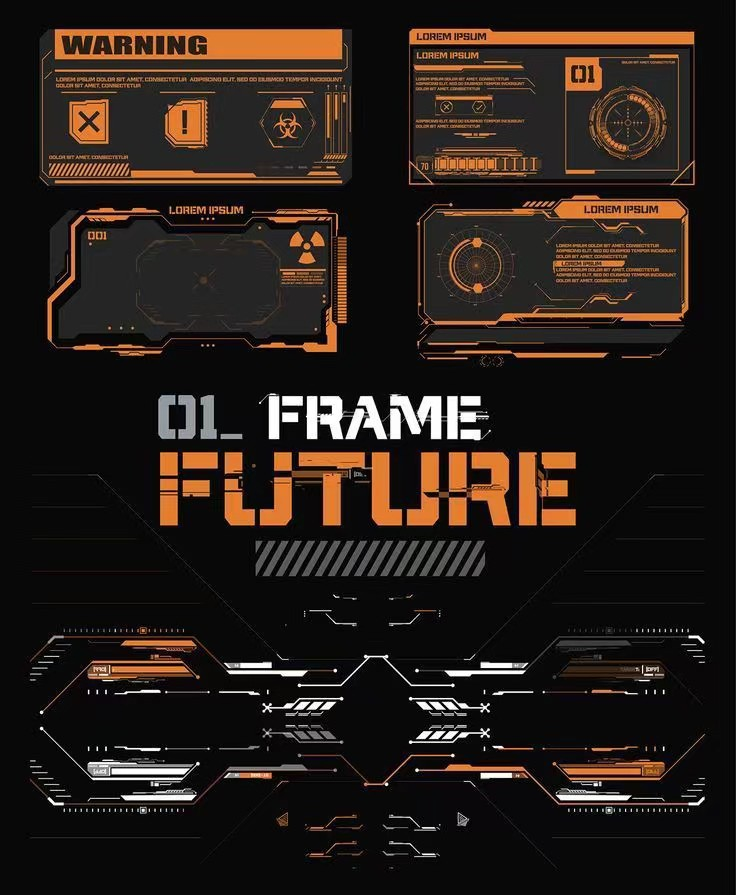
\includegraphics[scale=0.5]{material/UI设计参考2.jpeg}
				\caption{UI界面参考1}
			\end{figure}
			\begin{figure}[H]
				\centering
				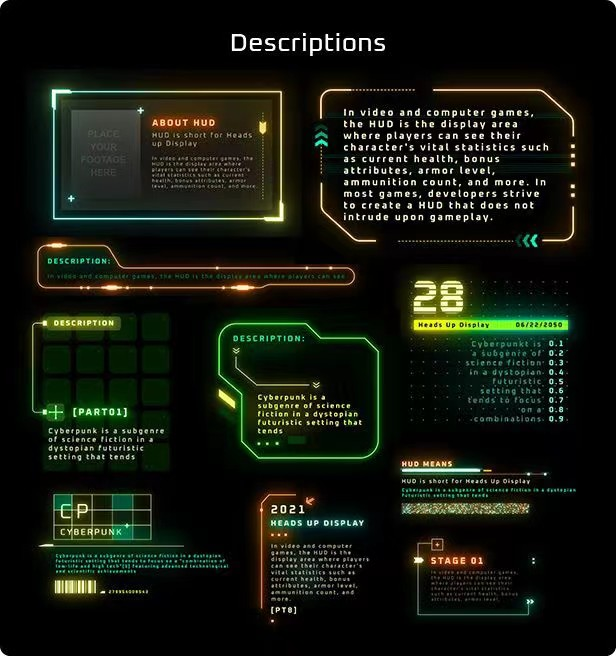
\includegraphics[scale=0.4]{material/UI设计参考3.jpeg}
				\caption{UI界面参考2}
			\end{figure}
			\begin{figure}[H]
				\centering
				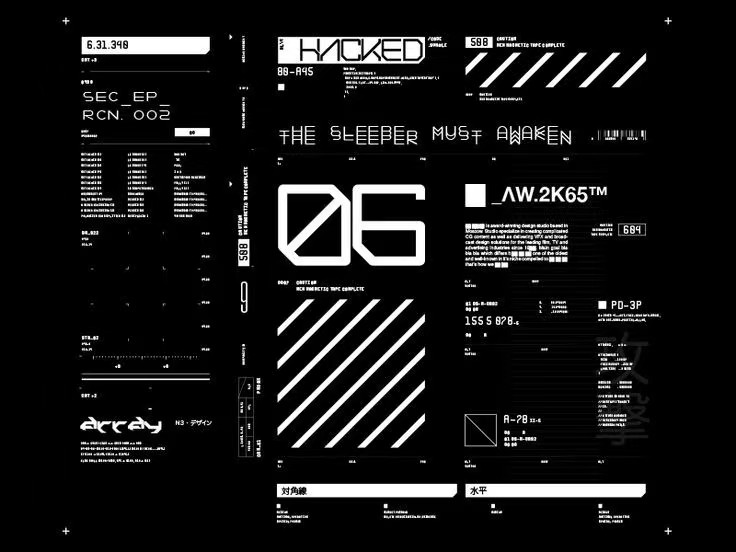
\includegraphics[scale=0.35]{material/UI设计参考4.jpeg}
				\caption{UI界面参考3}
				\label{UI简洁图}
			\end{figure}
			\subsubsection{游戏画面整体风格}
			\begin{figure}[H]
				\centering
				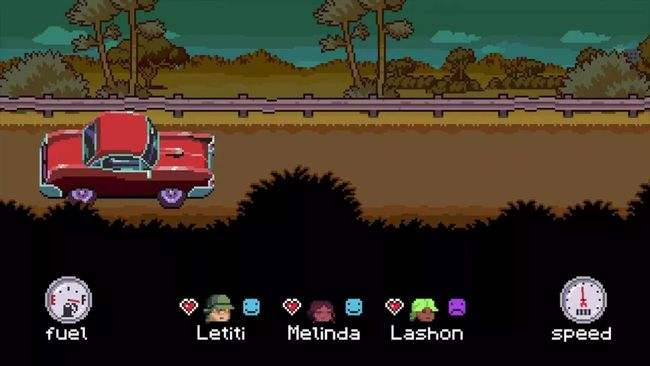
\includegraphics[scale=0.5]{material/DeathTripToCanada.jpeg}
				\caption{系统界面参考}
			\end{figure}
			\subsubsection{道具和UI}
			\begin{enumerate}
				\item 油量计已经画完了,食物的图还没有画
				\item NPC给的任务道具在背包里面的样子需要绘制,用低像素白色包边的方式画
				\item 警示UI的弹出方式应该是有科技感的激光弹出,而不是直接出现,当然如果时间不够的话可以直接用平移的方式来做,总之就是不要闪现出来
				\item 系统UI采用纯色、高对比度的形式,参考图\ref{UI简洁图},有简洁之美
				\item 角色的人物关系界面应该还要再画一遍人物的头像,这个使用低像素来做
			\end{enumerate}
	\section{剧情,对话设计}
		采用传统AVG的形式表达剧情,就是人物立绘+对话内容和选项,不需要制作场景和角色动画。可以参考图4。
		\subsection{序章}
			\begin{enumerate}
				\item 你在昏暗的飞行器内醒来,你坐在一个破旧的皮革坐垫上,周围的电子设备让你眼花缭乱
				\item “我是谁?我在哪?我要去哪里?”
				\item 似乎你的宇宙飞船遭受了陨石撞击,失去了记忆
				\item 还是看看周围,希望能回想起什么东西
				\begin{enumerate}
				\item 检查电子仪器-身边的设备因为经常被使用,已经十分破败了,并且你发现你能够不假思索的操控它们
				\item 检查身上装备-有一本破旧的笔记本,似乎是你的日记,可惜的是前面记载的东西已经模糊不清了,不过你可以在上面的空白处记上新的东西
				\item 试试回想过去-你闭上双眼,回忆自己的过去,伴随着阵阵刺痛,只想起一个宇宙航标,只要去往那里,或许就能恢复记忆,找到一切的解答
				\end{enumerate}
				\item 你站起身,在飞船的导航仪上标出了那个坐标的位置
				\item “真她妈远啊,就凭这小飞船真的能到那个地方吗?”
				\item 叹着气,你检查着飞船的物资情况,似乎想直接跃迁前往目标点并不现实,必须要在陌生星球、或是太空遗骸中进行物资补给
				\item “不仅是食物,连燃料也十分有限”--此时UI显示初始的资源数量
				\item 在空无一人的宇宙空间停滞不前可不是什么好主意,肯定会有未知的危险找上门来
				\item 该动身了....
			\end{enumerate}
			此时,结束对话界面,正式进入游戏操作界面。有UI界面解释。
			正式开始游戏进程。
		\subsection{因为物资不足而导致无法继续游戏}
			\begin{enumerate}
				\item “好,好饿”
				\item 你发疯般的在飞船的各个角落寻找任何可以吃的东西
				\item “没有,没有,没有,没有...什么都没有!”
				\item 你看着自己消瘦的躯体,大脑感受到阵阵晕眩
				\item 你感到自己站在路的中间,前路望不可及,向后望去已无后退之路
				\item “我好像一直萤火虫”
				\item 视线被黑雾充盈
				\item 游戏结束
			\end{enumerate}
		\subsection{因为燃料不足而导致无法继续游戏}
			\begin{enumerate}
				\item 你面前的油量表指针逐渐转向“0”刻度线
				\item 你慌张的望向存储燃油的油罐,只有罐壁上的痕渍证明着这里曾经存储过这飞船得以运作的流体
				\item 仪表盘上点亮的灯逐渐熄灭
				\item 一直以来被你所厌弃的换气扇的嗡嗡声也听了下来
				\item 一切都重归寂静
				\item 你在失去了重力维持装置的飞船中漂浮着
				\item 你在宇宙中作为某个恒星的卫星漂浮着
				\item 渺小的自我显然无法承载远大的理想,必然会被黑暗吞噬
				\item 游戏结束
			\end{enumerate}
		\subsection{终章}
			\begin{enumerate}
				\item 那只在幻想和地图上出现的行星第一次在飞船的舷窗上展示自己的姿态
				\item 虽然只是一个点,但随着飞船的逐渐靠近,点扩展成了球,成了面
				\item 随着飞船的靠近,你感到自己逐渐渺小
				\item 似乎这金黄的行星是宇宙的吞噬者,要把自己一口吞下
				\item 你来不及扫清“这里是否安全”的疑虑,操纵着飞船准备降落
				\item 触地回弹
				\item 剧烈的碰撞打乱了飞船上随意安置的设备,也让你大脑一阵晕眩,怀疑这一切是否真实
				\item 你摇了摇头,试图从这眩晕感中解脱出来,撞倒了一直准备着的宇航服,头盔似乎有所破裂
				\item 舱门开启,外面是金黄的草地,让你想到了家乡的麦地
				\item “啊啊啊,不知道母星的种植园,是否也有如此宏伟的麦浪”
				\item 你踏出一步,踩在这生机盎然的星球上,脚底触碰地面的柔软感,让你既熟悉又陌生
				\item 你仿佛初生的野兽般在地面上恣意奔跑,挥洒着自己用于应对危险的能量
				\item 你跑累了,倒在地上。忘我的啃噬地上的植被。
				\item 你到达了理想的彼岸!
				\item 可是,这值得吗?
			\end{enumerate}
		\subsection{真结局}
			\begin{enumerate}
				\item 母星,我回来了!
				\item 即使,您到了崩溃的边缘
				\item 即使,您身上布满重重创伤
				\item 即使,您的孩子并不爱惜您的一切
				\item 所以,我带着答案回来了
				\item 这漫长的旅途上,我经历了很多,也成长了很多,说是四处碰壁也不为过
				\item 脱离了您因质量而产生的引力,飞船的后方少了许多束缚,但前方却多了许多阻碍
				\item 但是,承受创伤正是长大的必经之路,当伤口愈合,我便成长一分
				\item 在这无期旅途中,有仇敌,也有朋友,虽然我的质量很小,但也有自己些微的引力,凝聚着趣味相投者
				\item 人的一生虽短暂,但出去走走也是值得的
				\item 可是,即使我到达那行星坐标之时,远在光年之外的您的引力,依旧把我和您紧紧的联系在一起
				\item 远去的游子,即使走的再远,也有回乡之时,我算是“少小离家老大回”也不为过
				\item 如今的我,以及不再是曾经那个只会依赖您的孩子了,身为“星孩”的我已经蜕变成了大人
				\item 我带着答案回来了,母星。
			\end{enumerate}
	\section{关卡、数值设计}
		\subsection{数值设计}
		\subsubsection{飞船油耗相关}
		\begin{enumerate}
			\item 飞船邮箱上限为100,之后可以通过强化扩建油箱来增大上限储量到200
			\item 初始飞船油箱的油在70~100不等
			\item 每进行一个回合,默认消耗油量为10点,即在不补充油的情况下可以支持10个回合的行动
			\item 在进入第二阶段的地图时,油量消耗增加到15点/回合
			\item 油箱扩建分为三个阶段,平均每一章可以升级一次,升级结果为120/140/200
		\end{enumerate}
		\subsubsection{飞船动力核心}
		飞船的动力核心无法被修复,并且有固定的耐久度,一旦飞船核心老化或是损坏那么玩家的游戏将直接失败。并且应该把核心耐久度直接的显示在主UI界面上。
		
		飞船的动力核心耐久度为40回合。返航解决会有NPC把自己飞船的动力核心拆下来给主角,所以可以有额外的动力返航。
		\subsubsection{食物消耗相关}
		\begin{enumerate}
			\item 飞船食物上限为50,不能扩建,但是可以溢出,溢出的食物只有4个回合的保鲜度,之后会损坏
			\item 食物可以被作为交易的一般等价物,遇到商人可以与之交易
			\item 正常消耗的食物为10点/回合,如果不获取食物的话只能支持5个回合的行动
			\item 食物的获取应该是溢出的,需要玩家利用溢出的食物进行交易
			\item 在初始10个回合内飞船内有食物的种植设备,可以将燃料以3:1向食物转化,但是需要一个回合的时间且不能把食物的数量增加到50以上。当10个回合,即新手保护期过了之后会遭遇小行星撞击,让培养装置损坏
			\item 完成NPC剧情奖励可以获得培养装置的修复工具
		\end{enumerate}
		\subsubsection{玩家属性相关}
			\begin{enumerate}
				\item 角色有生命值的隐性设定,连续受伤三次会直接去世
				\item 食物不足会降低角色的精神状态,并不会直接死亡,而是可以撑3个回合
				\item 角色可以通过休息来消耗额外的食物以及放弃探索机会来概率恢复受伤状态,或者使用治疗道具
				\item 当玩家不是满状态时,见到NPC的概率降低,发生不好的事件的概率增加
			\end{enumerate}
		\subsubsection{声望与结局与NPC}
			\begin{enumerate}
				\item 声望可以通过与NPC交流互动,以及某些探索事件来获取
				\item 声望的数量是NPC的好感度的体现,需要声望达到一定程度才能解锁NPC的后续剧情
				\item 声望到一个值才能算是得到所有NPC的信任,开启真结局的剧情
				\item 在探索时,玩家如果选择掠夺当地的物资,而不是交易之类的,就会减少声望
				\item 帮助探索时遇到的人就会提升声望,但是帮助纯粹的坏人是不会加声望的
				\item 当声望为负值时,即为加入邪恶阵营,掠夺有加成,并且不会收到海盗事件的影响
			\end{enumerate}
		\subsection{地图及事件设计}
		在总流程时间相对较长的情况下,逐个点来绘制地图显得有些困难。只需要根据回合和到达的位置来设定会发生的探索事件池就行,然后根据在某个地点探索的数量来绘制树状的地图,显示在仪表盘上。
		\subsubsection{地图的分区}
			参考文明6一局游戏150回合要玩7个小时左右,那么20个回合就差不多一个小时。考虑到操作数量的问题,本游戏应该回合会过的更快一点,因此设定直达回合数为25个回合,也就是说在不触发任何非强制事件的情况下需要25个回合的直线前进才能完成游戏。
			
			那么考虑到还需要玩家的探索需要花费回合数,大致完成时间为40个回合。
			
			前7个回合为新手教学区域,作为第一章,发生事件的概率小,给玩家更多的熟悉操作的时间。此时如果选择探索,那么基本都会得到资源的补给。当然,此区域探索次数过多,会有危险程度很高的事件发生。
			
			第8-第15回合NPC开始出现,事件的危险度开始增加,作为第二章。玩家在此应该会被初见杀。NPC不仅会有好人,也会有恶人出现,骗取同情和玩家的资源。并且此时飞船的推进器固定出现损坏,需要消耗更多的能源才能继续前进。
			
			第16-25回合,结束NPC剧情,飞船进入小行星带,危险度高的事件大幅增加并且难以获得探索收益。玩家进行结局的选择。
		\subsection{随机事件设计:大概需要30个} % TODO 做事件收益图
			\subsubsection{危险度无或者奖励事件}
			\begin{enumerate}
				\item 黑暗降临,世界陷入一片寂静,你在茫茫的宇宙中迷失了自我,呆呆的望向远方,一直望着,丝毫不觉时间流逝
				\item 你昏昏欲睡,此时飞船的舱门传来敲击声,你做好全副武装后打开舱门后发现,是被遗弃的补给仓撞上了飞船,虽然让你心惊胆战了一阵,好在补给仓里还有剩余的资源能够安抚你的心灵。(燃油+10,食物+10)
				\item 飞船遭受了电磁风暴袭击,所有的电子设备都被破坏,通讯被中断,导航也失效了。你在更换了部分备用零件之后,系统终于正常运行了起来。
			\end{enumerate}
			\subsubsection{危险度低:1-2}
			\begin{enumerate}
				\item 飞船的燃油舱突然泄漏,刺耳的警报声向你反复强调着珍贵的燃料被无端消耗着,幸好维修的及时,挽回了部分损失。(燃油-10)
				\item 扭曲的太空蠕虫将自己的身体吸附在你的飞船之上,似乎把此地当成了安全的避风港。显然,你飞船的质量无法支撑携带这些“额外乘客”,只好向外丢弃一些食物来引走它们。(食物-5,燃油-5)
				\item 一群星际强盗正在劫掠一艘过路的飞船,你要去帮助他们吗?
					\begin{enumerate}
					\item 选择帮忙:路见不平当然要拔刀相助,你操纵着飞船向海盗们飞去,海盗的反击让你的飞船收到了损伤,但是你凭借自己的经验进行了激烈的反击,最后还是获得了胜利。海盗们仓皇逃窜(燃油-15,声望+10)
					\item 选择不帮忙:多一事不如少一事,还是快走吧
					\end{enumerate}
				\item 飞船与太空垃圾发生了直接性的撞击!赶紧操纵飞船躲避接连不断的碎块撞击(燃油-20)
				\item 
			\end{enumerate}
			\subsubsection{危险度中:3-4}
			\begin{enumerate}
				\item 飞船遭受了小行星冲击,你紧急关闭了飞船的自动驾驶,手动操纵飞船躲避向你袭来的致命石块,即使如此,飞船也遭受重创,并且消耗了比平常更多的燃料。(10回合离开新手区域后固定发生,损坏推进器、植物培养装置。燃油-20)
				\item 宇宙之夜并不宁静,往往在你有所懈怠之时遭遇危险之事。一队全副武装的星际海盗在你小憩之时登上了你的飞船,试图劫掠你赖以维生的资源。你奋起反抗,才勉强将他们击退,可是已经被抢走的资源已经回不来了。(燃油-30,食物-20)
				\item 飞船的燃料突然泄漏,在维修完成前还是有大量的燃料被抛洒到了太空之中(燃油-30)
				\item 飞船中储存的食品在宇宙射线的辐射之下发生了变质,贸然吃下可能会发生不好的事情,还是赶快丢弃吧(食物-15)
			\end{enumerate}
			\subsubsection{危险度高:5}
			\begin{enumerate}
				\item 遇到了强烈的恒星风暴袭击,飞船的温度控制终端失联,能量核心失去束缚(核心耐久-3)
			\end{enumerate}
		\subsection{探索事件设计:大概需要20个}
			探索事件分为三个区域,分别对应第一章至第三章的地图,并且探索事件是不重复出现的,为了防止在同一个地点一直拖着不前进的情况出现。
			当有NPC事件可以触发的时候,默认触发NPC事件,如果没有NPC事件触发,才会有普通探索事件出现
			\subsubsection{第一章}
				\begin{enumerate}
					\item 发现了罕见的彗星碎片,蕴含的寒冰能量可以延长食物的保存时间!(冰箱外的食物保鲜3个回合)
					\item 远处的黑影竟然是废弃的飞船,上面说不定会有遗弃者留下的资源!(食物+5,燃油+5)
					\item 在穿越危机重重的小行星带后,一无所获(燃料-10)--当所有回合都走完之后默认是这个
					\item 栽培仓内的作物在经受宇宙射线的照射后,发生了正面变异(食物+10)
					\item 捡到了不明机械设备的零件,可以用来给油箱扩容(油箱容量上限变成120)
					\item 遇到了星际中的游荡商人,用食物可以2:1交换燃料,3:1燃料交换食物
				\end{enumerate}
			\subsubsection{第二章}
			\subsubsection{第三章}
		\subsection{NPC及其任务线设计:13个(暂定)} % TODO 剧情这边得看书来学,不然他妈写不好故事
		设定为以古代神话传说中神的角色来命名NPC,并且根据NPC的名字来设计相似的任务线路,但本质还是给主角的航行提供一些路线上的帮助和建立同主角的羁绊。% 这边就可以使用学到的电影剧作中的任务来设计角色,但是不好弄
			\subsubsection{科技:厄佩博士Dr.Epi}
			\textbf{人物设定} 
			\begin{enumerate}
				\item 在一开始就能遇到,主要是提供教程类的NPC,厄佩博士会告诉玩家关于飞船的细节,以及对游戏的科技树背景作介绍
				\item 厄佩博士加入这场太空逃亡的原因是主要的研究方向是传统燃料推进飞船,而这种飞船已经被全线淘汰,博士被开除出研究院,因为负担不起高额的“人口保障费”,选择驾驶自己的燃料飞船逃亡
				\item 厄佩博士对于自己的生命并不在意,冒着必死的觉悟离开不需要自己的世界,并且与自己的飞船一同在宇宙消亡而不是作为战犯或是战俘牺牲
				\item 厄佩博士会向玩家讨要燃料和食物,作为回报他会告诉玩家一些信息
				\item 厄佩博士不会让任何人靠近他的船,但是在真结局返航时刻厄佩是第一个选择把自己的船拆了装在主角的飞船上的“这是他最好的归宿”,然后自尽
				\item 厄佩博士是唯一会在全部的时间段遭遇的NPC,他的任务线即教程任务线,在第一次探索时一定会碰到他
			\end{enumerate}
			\textbf{任务线设定}
			\begin{enumerate}
				\item 博士在用多种频道的无线电波求救,请求有人来施舍一些食物和燃油
					\begin{enumerate}
					\item 主角选择前往->失去10燃油10食物,声望+20->博士讲述战乱的背景以及自己逃亡原因,如果此时主角的飞船动力系统还没坏,那么就指出动力系统在将来的某个时刻会坏掉,如果已经坏了,就指出自己会修,但是需要准备材料才行
					\item 主角选择忽视,并且继续前进->厄佩博士死亡,任务线终结 
					\end{enumerate}
				\item 主角在探索小行星的时候再次与厄佩博士相遇,厄佩博士正在采集星球上的资源,并且指出这就是飞船核心的必要组成部分,以目前被禁止了的燃料动力飞船的发展进度,是不能够再次建造新的飞船的,所以燃料飞船的总量会逐渐减少,即使用大量的资源去修复已有的飞船核心也无法逆转破损的注定局面,自己的逃亡之旅终将以冰冷的宇宙空间作结(声望+20,燃油+10)
				\item 厄佩博士向周围发出了大功率求救信号,却不知道自己的行为会引来贪婪而冷血的星际旅行者,但碰巧的是,你也收到了这个大功率求救信号。
					\begin{enumerate}
					\item 选择在远处屏蔽信号的传播,防止吸引其他掠夺者(声望+10)
					\item 选择前往信号所在的地点,看看究竟发生了什么->厄佩博士的飞船因为遭受小行星的撞击,完全失去动力,并且外部装甲大量损坏只能通过向外发送求救信号来获取帮助,主角选择帮助厄佩博士修复飞船(燃油-20,需要在3个回合内进行探索找到修复飞船所需的材料,声望+10)
					\end{enumerate}
				\item 当主角触发危险度为3及以上的探索事件时,厄佩博士会出现帮助你分摊一半的损失,以此报答你的救命之恩,向主角的行为表示感谢
			\end{enumerate}
			\subsubsection{神谕:福柏Phobe}
			\subsubsection{收获:墨诺Meno}
			\subsubsection{战斗:布拉吉Brage}
			\subsubsection{精神:忒弥斯Themis}
			\subsubsection{生命:奎特Qetesh}
			\subsubsection{神秘:阿斯图Astru}
			\subsubsection{自然:维达Vida}
			\textbf{人物设定}
			\begin{enumerate}
				\item 是注定失败的领袖,但是有着绝对优秀的个人魅力,只是因为理念不同而走上了错误道路。是旧时代的代表性人物
				\item 战斗型的角色,在主角追随他,作为他的部下的情况下才可以推动剧情
				\item 可以参考《三体》中的韦德
				\item 这边需要注意的是,对于即将进入交战区的描写需要提前几个回合弄点铺垫
			\end{enumerate}
			\textbf{任务线设定}
			\begin{enumerate}
				\item 主角的飞船需要经过一片交战区,电磁炸弹影响了飞船的导航系统,你在不由己的情况下进入了交战区内部,迷失了方向。四处溅射的激光束,封锁了你前进的道路,一切轻举妄动似乎都会吸引这群草木皆兵的战士们。(下一次行动只能选择探索)
				\item 战斗似乎进入了停火期,炫目的激光也少了很多,此时你的无线电传来消息,让你跟随指示的路线前进即可安全离开交战区。那是一个男人的声音,自称“维达”。成功离开后,你想向他表示感谢,可是发送的消息却再也没有回复(声望+10)
				\item 主角在探索时遇到了一架飞船停靠在逐渐熄灭的恒星边上,似乎是想要收集聚变能量而不小心被恒星引力俘获,无法逃离
					\begin{enumerate}
						\item 多一事不如少一事,直接离开(声望-20,维达任务线直接结束)
						\item 给予燃料,让飞船拥有更大动力来脱离引力束缚(燃料-10,声望+10)
						\item 用自己的飞船牵引,帮助脱离引力束缚(燃料-10,核心耐久-1,声望+20)
					\end{enumerate}
				\item 维达希望主角帮助反抗军找到三处补给站(就是探索的时候出现的加燃料和食物的东西),并且把信标发给维达,成功后维达会重新组织反抗军$\rightarrow$完成真结局维达来帮忙的条件1
				\item 玩家在进行普通探索的时候,有几率找到军用无线电设备,可以拆了变成零件维修飞船(核心耐久+1),也可以选择给维达,支援反抗军的行动(声望+20)
				\item 韦德联系主角,发现了政府军给养母舰的维护设施,希望主角靠近设施,在没人注意的时候发射激光引导反抗军的导弹
					\begin{enumerate}
						\item 选择帮忙,炸毁了设施,但是主角协助反抗军被证明
						\item 选择把瞄准设备指向维达的母舰,反抗军势力被大幅度削减,主角被表扬
						\item 什么也不做,反抗军再次爆发正面冲突,反抗军进度被减缓
					\end{enumerate}
			\end{enumerate}
			\subsubsection{虚无:伊米尔Ymer}
			\subsubsection{欺诈:海德拉Hydra}
			\subsubsection{情欲:塞壬Siren}
			\subsubsection{愤怒:芬克斯phinx}
			\subsubsection{贪婪:俄泽斯Oizys}
		\section{制作方案以及制作时间规划}
			\subsection{用PPT做项目交互很演示}
			因为没有战斗方向的设定,ppt就能直接的展示交互的效果,并且能够使用到之前画的相关的素材,操作难度十分低,当然,屏幕设定需要和实机运行相同
			\subsection{使用虚幻引擎进行游戏demo制作}
			demo阶段考虑使用虚幻引擎进行制作,以下为优势分析
			\begin{enumerate}
				\item 是课程相关内容,有老师可以直接问,同学也可以直接帮忙
				\item 有项目开发经验,之前的肌肉记忆还在,并且可以看之前的笔记什么的
				\item 有像素游戏的制作先例《幻想乡萃夜祭》,也是用虚幻做的
				\item 蓝图,省略编程步骤,但是用git进行协同编辑不太好用,不过也不用协同编辑,草
				\item godot也能做,但是网上教程少,unity基本没有经验,虽然教程多,但是需要很多时间学习
			\end{enumerate}
			\subsection{初步时间安排}
				具体时间还需要和美术商谈下,如果在找不到美术的情况下就使用novelai画图,那这样就必须放弃全局像素画的想法了,根据现实情况在进行取舍。demo就做到离开新手区域,不需要很多东西,但是需要精致,有成品的水平,而不是赶进度他妈的。
				
				项目管理可以使用flowus或者是github的工作流程图表,时间很充裕,重要的是能够坚持做下去,需要保持热情。
				
				11月把项目的策划全部写完,并且有空闲的情况下画画像素画,但也其实做不到一个文档干到底的情况,只能说完成个大概
				
				12月即使没有美术,也要用自己做的素材尝试进行工程的构建了
				
				1月份正式开搞,完了debug
		
\end{document}